\documentclass[aspectratio=169,11pt,t]{beamer}
\input{../../../../theme/ksa-cs-v2.tex}
% 원본 덱 (ksa-theme): slides/v2/ml1/week04/em_algorithm/ -- 그림은 거기 figs/ 를 그대로 쓴다
\setbeamerfont{author}{size=\normalsize}
\setbeamerfont{institute}{size=\small}
\graphicspath{{figs/}{../../../../v2/ml1/week04/em_algorithm/figs/}{../../../../assets/}}
\makeatletter
\newcommand{\markpage}[1]{\protected@write\@auxout{}{\string\newlabel{#1}{{\the\c@framenumber}{}}}\hypertarget{#1}{}}
\newcommand{\pref}[1]{\hyperlink{#1}{\textcolor{ksagolddk}{(p.\ref{#1})}}}
\makeatother

\renewcommand{\ksacredit}{Machine Learning and Deep Learning \,\textperiodcentered\, EM 알고리즘}
\title{EM 알고리즘 (Expectation-Maximization)}
\subtitle{모르는 것은 확률로 채우고, 다시 고치고}
\author{Machine Learning and Deep Learning}
\institute{한국과학영재학교 (KSA)}
\date{}
\begin{document}
{\setbeamertemplate{footline}{}\begin{frame}[c,noframenumbering]\titlepage\end{frame}}

\section{질문}
% --- 오늘의 질문
\begin{frame}{오늘의 질문}
\vfill
\centering\includegraphics[width=0.8\linewidth]{em_hook.png}\par\vskip0.4em
{\Large 학년이 지워진 키 명단 24명}\\[0.4em]
{\large 초등 6학년 몇 명과 중학 3학년 몇 명이 섞여 있다. \kq{누가 초6이고 누가 중3일까?}}
\vfill
\note{학생 24명의 키 명단입니다. 원래는 초등학교 6학년과 중학교 3학년이 섞여 있었는데, 학년 칸이 지워졌습니다. 키만 보고 누가 초6이고 누가 중3인지 맞힐 수 있을까요? 키가 작은 쪽은 초6, 큰 쪽은 중3일 것 같지만, 155에서 160 사이는 애매합니다. 그리고 몇 명씩인지도 모릅니다. 지난 시간의 k-means처럼 라벨 없이 무리를 나누는 문제인데, 오늘은 애매함까지 확률로 다루는 방법을 배웁니다.}
\end{frame}

\section{모델}
% --- 닭과 달걀
\begin{frame}{닭이 먼저냐 달걀이 먼저냐}
\vfill
\centering
{\Large 무리를 알면 \quad $\to$ \quad 무리마다 평균 · 표준편차를 구할 수 있다}\\[0.8em]
{\Large 평균 · 표준편차를 알면 \quad $\to$ \quad 학생마다 어느 무리인지 정할 수 있다}\\[1.2em]
{\large 그런데 \kq{둘 다 모른다} \quad $\to$ \quad 하나를 대충 정하고, 번갈아 고친다}\\[0.6em]
{\small 지난 시간 k-means 도 같은 구조: 할당 $\leftrightarrow$ 갱신}
\vfill
\note{이 문제는 닭이 먼저냐 달걀이 먼저냐입니다. 누가 초6인지 알면 초6의 평균 키를 바로 구할 수 있습니다. 반대로 초6과 중3의 평균 키를 알면 학생마다 어느 쪽에 가까운지로 학년을 정할 수 있습니다. 그런데 우리는 둘 다 모릅니다. 그래서 하나를 대충 정해 놓고, 다른 하나를 구하고, 다시 처음 것을 고치는 일을 번갈아 합니다. 지난 시간 k-means의 할당과 갱신이 정확히 이 구조였습니다. EM은 여기서 할당을 0과 1이 아니라 확률로 합니다.}
\end{frame}

% --- 모델
\begin{frame}{모델: 가우시안 두 개를 섞은 분포}
\markpage{gmm}
\vfill
\centering
{\LARGE\[ p(x) = \textcolor{ksablue}{\pi_1}\,\mathcal{N}(x;\ \mu_1, \sigma_1^2) + \textcolor{ksared}{\pi_2}\,\mathcal{N}(x;\ \mu_2, \sigma_2^2) \]}\vskip0.6em
\renewcommand{\arraystretch}{1.3}
{\large\begin{tabular}{ll}
$\mu_j, \sigma_j$ & 무리 $j$ 의 평균 · 표준편차 (가우시안 시간의 종 하나)\\
$\pi_j$ & 무리 $j$ 의 비율 \quad ($\pi_1 + \pi_2 = 1$)\\
잠재변수 $z$ & 학생마다 숨어 있는 학년 \quad (데이터에 없다)
\end{tabular}}\vskip0.4em
{\small 가우시안 혼합 모델 (Gaussian Mixture Model, GMM). 정할 숫자: $\mu_1, \mu_2, \sigma_1, \sigma_2, \pi_1, \pi_2$}
\vfill
\note{먼저 모델을 정합니다. 학년마다 키가 가우시안 종 모양이라고 가정하면, 전체 명단은 종 두 개를 섞은 분포입니다. 파이는 각 무리의 비율입니다. 초6이 절반이면 파이 1이 0.5입니다. 학생마다 숨어 있는 학년을 잠재변수 z라고 부릅니다. 데이터에는 없지만 분명히 있는 값입니다. 이런 모델을 가우시안 혼합 모델, GMM이라고 하고, 우리가 정해야 할 숫자는 평균 둘, 표준편차 둘, 비율 둘, 모두 여섯 개입니다.}
\end{frame}

\section{E · M}
% --- E 단계
\begin{frame}{E 단계: 학생마다 확률 매기기}
\markpage{estep}
\vfill
\centering\includegraphics[width=0.6\linewidth]{em_estep.png}\par\vskip0.1em
{\normalsize\[ \gamma_{i2} = \frac{\pi_2\,\mathcal{N}(x_i;\mu_2,\sigma_2^2)}{\pi_1\,\mathcal{N}(x_i;\mu_1,\sigma_1^2) + \pi_2\,\mathcal{N}(x_i;\mu_2,\sigma_2^2)} \qquad
153\text{ cm}: \; \frac{0.5 \cdot 0.0629}{0.5 \cdot 0.0587 + 0.5 \cdot 0.0629} = 0.52 \]}
\vfill
\note{시작은 아무렇게나 합니다. 평균을 150과 155, 표준편차는 둘 다 6, 비율은 반반으로 찍었습니다. 첫 번째 단계는 E 단계, 기댓값 단계입니다. 학생마다 어느 무리일지 확률을 매깁니다. 가우시안 시간에 키로 남녀를 맞힐 때 쓴 베이즈 정리와 똑같습니다. 153센티에서 155짜리 종의 높이는 0.0629, 150짜리 종은 0.0587입니다. 비율 0.5를 곱해 나누면 중3일 확률 0.52, 거의 반반입니다. 이 확률을 책임값, 감마라고 부릅니다. 그림에서 색이 파랑에서 빨강으로 갈수록 중3일 확률이 큽니다.}
\end{frame}

% --- M 단계
\begin{frame}{M 단계: 확률을 무게로 다시 구하기}
\markpage{mstep}
\vfill
\centering\includegraphics[width=0.62\linewidth]{em_mstep.png}\par\vskip0.1em
{\large\[ \mu_j = \frac{\sum_i \gamma_{ij}\,x_i}{\sum_i \gamma_{ij}} \qquad
\sigma_j^2 = \frac{\sum_i \gamma_{ij}\,(x_i - \mu_j)^2}{\sum_i \gamma_{ij}} \qquad
\pi_j = \frac{1}{m}\sum_i \gamma_{ij} \]}
{\large 평균 150 · 155 $\to$ \kb{152 · 162} \qquad 비율 0.5 · 0.5 $\to$ 0.35 · 0.65}
\vfill
\note{두 번째 단계는 M 단계, 최대화 단계입니다. E 단계에서 매긴 확률을 무게로 써서 평균, 표준편차, 비율을 다시 구합니다. 153센티 학생은 초6 쪽 평균에 0.48만큼, 중3 쪽 평균에 0.52만큼 들어갑니다. 가우시안 시간의 평균, 분산 식에서 그냥 더하던 것을 무게를 곱해 더하는 것으로 바꾼 것뿐입니다. 그 결과 평균은 152와 162로 벌어졌고, 비율은 0.35와 0.65가 됐습니다. 아직 큰 학생 쪽이 많다고 보고 있습니다.}
\end{frame}

% --- k-means 와 비교
\begin{frame}{k-means 와 무엇이 다른가}
\vfill
\centering
\renewcommand{\arraystretch}{1.6}
{\large\begin{tabular}{lll}
 & k-means & EM (GMM)\\\hline
할당 & 가장 가까운 무리에 \textbf{0 또는 1} & 무리마다 \kb{확률} $\gamma$ (합 1)\\
갱신 & 맡은 점의 평균 & 확률을 무게로 한 평균 · \textbf{표준편차} · \textbf{비율}\\
무리 모양 & 둥글고 크기가 비슷하다고 가정 & 폭 ($\sigma$) 과 크기 ($\pi$) 도 배운다\\
결과 & ``이 학생은 중3'' & ``이 학생은 중3일 확률 60\%''
\end{tabular}}
\vfill
\note{지난 시간 k-means와 나란히 놓으면 차이가 분명합니다. k-means는 각 점을 가장 가까운 무리 하나에 0 아니면 1로 넣습니다. EM은 무리마다 확률을 줍니다. 갱신할 때 k-means는 평균만 옮기지만, EM은 확률을 무게로 평균뿐 아니라 표준편차와 비율까지 다시 구합니다. 그래서 무리마다 폭과 크기가 달라도 따라갈 수 있습니다. 결과도 이 학생은 중3이다가 아니라 중3일 확률 60퍼센트처럼 애매함을 그대로 남깁니다. 표준편차를 모두 같게 고정하고 확률을 0과 1로 반올림하면 EM이 k-means가 됩니다.}
\end{frame}

\section{반복}
% --- 반복
\begin{frame}{E · M 을 반복하면}
\vfill
\centering\includegraphics[width=0.6\linewidth]{em_traj.png}\par\vskip0.2em
{\large 40번 반복 $\to$ 평균 \kb{150 · 165} \quad (진짜 151 · 167, 학년은 한 번도 안 봤다)}
\vfill
\note{E 단계와 M 단계를 40번 반복했습니다. 두 평균이 점점 벌어져 150과 165센티에 자리 잡고 거의 움직이지 않습니다. 실제 초6과 중3의 평균은 151과 167입니다. EM은 학년 정보를 한 번도 보지 않았는데 거의 맞혔습니다. 표준편차는 4.3과 5.8, 비율은 0.43과 0.57이 됐습니다.}
\end{frame}

% --- 우도
\begin{frame}{반복할수록 더 그럴듯해진다}
\markpage{ll}
\vfill
\centering\includegraphics[width=0.41\linewidth]{em_ll.png}\par\vskip0.2em
{\Large\[ \log L = \sum_{i=1}^{m} \log p(x_i) \quad : \quad -103.1 \to -87.5 \to \cdots \to \kb{-85.8} \]}
{\small 로그 우도 = 지금 모델에서 이 명단이 나올 확률의 로그. EM 은 이 값을 \textbf{한 번도 줄이지 않는다} (k-means 의 SSE 와 같은 성질)}
\vfill
\note{EM이 무엇을 좋게 만들고 있는지 봅시다. 지금 모델에서 이 명단 24명의 키가 나올 확률, 즉 우도에 로그를 씌운 값입니다. 처음 마이너스 103.1에서 한 번 반복하면 마이너스 87.5로 크게 오르고, 마지막에는 마이너스 85.8에서 멈춥니다. 중요한 성질은 EM이 이 값을 한 번도 줄이지 않는다는 겁니다. k-means의 SSE가 한 번도 늘지 않았던 것과 같습니다. 그래서 반드시 어딘가에서 멈추고, 역시 시작에 따라 지역 최댓값에 멈출 수 있습니다.}
\end{frame}

% --- 결과
\begin{frame}{결과: 확실한 학생과 애매한 학생}
\markpage{final}
\vfill
\centering\includegraphics[width=0.6\linewidth]{em_final.png}\par\vskip0.1em
{\large 0.5 로 나누면 \kb{24명 중 22명} 정답 \quad 틀린 둘: 157 cm (중3 \kq{60\%}), 159 cm}\\[0.2em]
{\small 157 cm 는 실제 초6. EM 은 ``중3 60\%'' 로 애매함을 남겼다 $\to$ 0.5 근처는 다시 확인}
\vfill
\note{40번 반복한 뒤의 결과입니다. 아래 막대는 학생마다 중3일 확률입니다. 작은 학생은 0, 큰 학생은 1로 확실합니다. 0.5를 기준으로 나누면 24명 중 22명이 실제 학년과 맞습니다. 틀린 둘은 157센티와 159센티 학생인데, 둘 다 실제로는 초6입니다. 키가 중3 무리와 겹치는 곳에 있으니 키만으로는 사람도 틀릴 만합니다. 중요한 건 EM이 157센티를 중3이라고 단정하지 않고 중3일 확률 60퍼센트라고 했다는 점입니다. 확률이 0.5 근처인 학생은 다른 정보로 다시 확인하면 됩니다.}
\end{frame}

\section{다른 분포}
% --- 푸아송 혼합
\begin{frame}{가우시안만이 아니다: 푸아송 두 개 섞기}
\markpage{poisson}
\vfill
\begin{columns}[c]
\column{0.52\linewidth}\centering
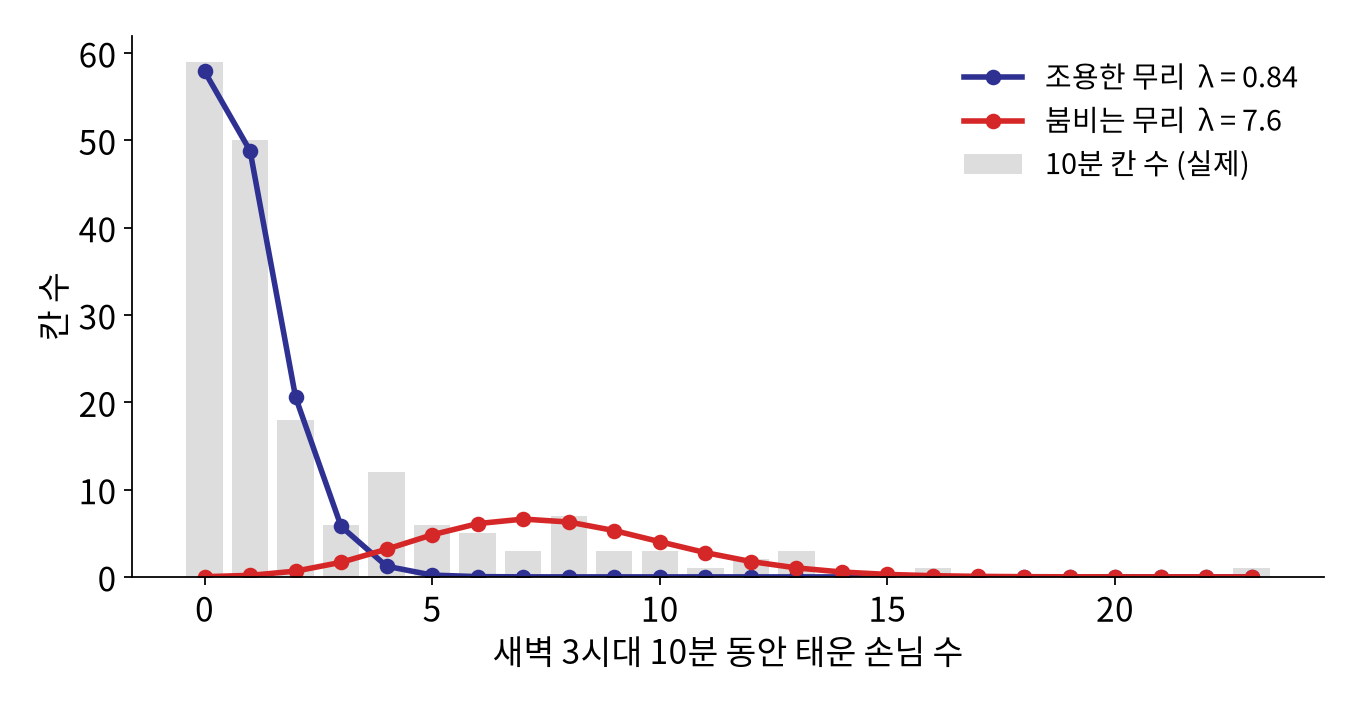
\includegraphics[width=\linewidth]{em_poisson.png}\\
{\small 뉴욕 택시 Gramercy 구역, 2024년 1월 새벽 3시대 10분 칸 180개}
\column{0.46\linewidth}
{\large 개수 데이터 $\to$ 무리마다 \textbf{푸아송}}\\[0.2em]
{\Large $\displaystyle P(k) = \frac{\lambda^k e^{-\lambda}}{k!}$}\\[0.6em]
{\large \kb{E}: 종의 높이 대신 푸아송 확률로 $\gamma$}\\[0.2em]
{\small 예: 3명 $\to$ 조용 0.043, 붐빔 0.037\\ \quad 비율 0.75 · 0.25 $\to$ 붐빌 확률 \textbf{22\%}}\\[0.6em]
{\large \kb{M}: 무게를 곱한 평균이면 끝}\\[0.2em]
{\Large $\displaystyle \lambda_j = \frac{\sum_i \gamma_{ij}\, x^{(i)}}{\sum_i \gamma_{ij}}$}\\[0.6em]
{\small 요일은 지우고 손님 수만 넣었다}
\end{columns}
\vfill
\note{EM은 가우시안에만 쓰는 게 아닙니다. 개수를 세는 데이터에는 분포 시간에 본 푸아송을 무리마다 두면 됩니다. 뉴욕 옐로 택시의 실제 기록에서, 그래머시라는 구역에서 2024년 1월 새벽 3시대에 10분마다 손님을 몇 명 태웠는지 센 180칸입니다. 요일 정보는 지우고 손님 수만 넣었습니다. E 단계는 종의 높이 대신 푸아송 확률로 칸마다 무리 확률을 매깁니다. 예를 들어 3명을 태운 칸은 조용한 무리에서 나올 확률이 0.043, 붐비는 무리에서 0.037이고, 비율 0.75와 0.25를 곱해 베이즈 정리로 나누면 붐비는 무리일 확률이 22퍼센트입니다. M 단계는 더 쉽습니다. 람다는 그 확률을 무게로 곱한 평균, 이게 끝입니다. 반복하면 그림처럼 조용한 무리는 람다 0.84, 붐비는 무리는 7.6으로 갈라집니다.}
\end{frame}

% --- 결과 확인
\begin{frame}{숨은 값은 무엇이었나: 요일}
\vfill
\centering
\renewcommand{\arraystretch}{1.5}
{\large\begin{tabular}{lccc}
 & 조용한 무리 $\lambda$ & 붐비는 무리 $\lambda$ & 붐비는 비율\\\hline
EM (손님 수만 보고) & 0.84 & 7.6 & 25\%\\
정답 (요일로 나눠 보면) & 평일 새벽 0.80 & \kb{주말 새벽} 7.35 & 27\% \;(48 / 180)
\end{tabular}}\vskip0.6em
{\large 180칸 중 \kb{173칸 (96\%)} 을 요일과 같게 나눴다 \quad 숨은 값 = 금 · 토요일 밤}\\[0.8em]
{\large 규칙: 무리마다 어떤 분포든 두고, \textbf{M = 무게를 곱한 최대우도}}\\[0.2em]
{\small 가우시안이면 평균 · 분산, 푸아송이면 평균}\\[0.2em]
{\small \textbf{t 분포 혼합}: 튀는 값에 덜 휘둘리는 군집 (Peel \& McLachlan, 2000)}
\vfill
\note{EM이 찾은 두 무리는 무엇이었을까요? 지워 둔 요일을 다시 붙여 보면, 조용한 무리는 평일 새벽으로 평균 0.80명, 붐비는 무리는 주말 새벽으로 평균 7.35명, 비율 27퍼센트입니다. EM이 찾은 0.84, 7.6, 25퍼센트와 거의 같습니다. 180칸 중 173칸, 96퍼센트를 요일과 같게 나눴습니다. 숨은 값은 금요일과 토요일 밤, 술집에서 집에 가는 사람들이었던 거죠. 규칙은 하나입니다. 무리마다 어떤 분포든 두고, M 단계에서는 그 분포의 최대우도 추정을 무게를 곱해서 하면 됩니다. 가우시안이면 평균과 분산, 푸아송이면 평균입니다. 스튜던트 t 분포를 섞을 수도 있습니다. 꼬리가 두꺼워서 멀리 튄 값에 덜 휘둘리는 군집이 되는데, 점마다 숨은 값이 하나 더 늘 뿐 같은 E, M 반복입니다.}
\end{frame}

% --- 어디에 쓰나
\begin{frame}{EM 은 어디에 쓰나: 숨어 있는 값이 있을 때}
\vfill
\centering
\renewcommand{\arraystretch}{1.5}
{\large\begin{tabular}{ll}
\textbf{클러스터링} & 오늘처럼 GMM: 무리 (학년) 가 숨어 있다\\
\textbf{결측치} & 빈칸을 확률로 채우고 모델을 고치고 반복\\
\textbf{번역 (1990년대)} & 사전 없이 문장 쌍만으로 단어 짝 맞추기 (IBM Model 1)\\
\textbf{음성 인식 · 유전체} & 숨은 마르코프 모델 (HMM) 학습 (Baum-Welch)
\end{tabular}}\vskip0.8em
{\large 공통점: 모르는 값을 \kb{확률로 채우고 (E)}, 그걸로 \kb{모델을 고친다 (M)}}
\vfill
\note{EM은 클러스터링에만 쓰이는 게 아닙니다. 데이터에 숨어 있는 값이 있을 때마다 쓰입니다. 결측치가 있으면 빈칸을 확률로 채우고 모델을 고치기를 반복합니다. 1990년대 통계 번역은 사전 없이 영어와 프랑스어 문장 쌍만 보고 어떤 단어끼리 짝인지를 EM으로 배웠습니다. 음성 인식과 유전체 분석의 숨은 마르코프 모델도 EM으로 학습합니다. 공통점은 모르는 값을 확률로 채우는 E 단계와, 그걸로 모델을 고치는 M 단계입니다.}
\end{frame}

\section{연습}
% --- 문제풀이
\begin{frame}{문제풀이}
\vfill
\begin{enumerate}
\item 키 160 cm 에서 두 종의 높이가 0.02 (초6), 0.06 (중3), 비율이 0.5 · 0.5 이다. E 단계의 중3 확률은? 비율이 0.75 · 0.25 라면?\vskip0.8em
\item 점 2개: $x = 0$ ($\gamma = 0.9$), $x = 10$ ($\gamma = 0.1$) 가 무리 1 에 속할 확률. M 단계에서 무리 1 의 평균은?\vskip0.8em
\item EM 을 다른 시작점으로 두 번 돌렸더니 로그 우도가 $-90$, $-86$ 이었다. 어느 결과를 쓰나? 이유는?\vskip0.8em
\item 모든 $\sigma$ 를 같게 고정하고, $\gamma$ 를 0 또는 1 로 반올림하면 EM 은 무엇이 되나?\vskip0.8em
\item 푸아송 혼합: 칸 2개 $x = 0$ ($\gamma = 0.2$), $x = 10$ ($\gamma = 0.8$) 가 붐비는 무리일 확률. M 단계의 붐비는 무리 $\lambda$ 는?
\end{enumerate}
\vfill
\note{1번 답. 반반이면 0.06 나누기 0.08, 0.75입니다. 비율이 0.75와 0.25면 초6 쪽 0.015, 중3 쪽 0.015라서 0.5, 반반이 됩니다. 2번 답. 0.9 곱하기 0 더하기 0.1 곱하기 10을 0.9 더하기 0.1로 나누면 1입니다. 3번 답. 로그 우도가 큰 마이너스 86입니다. 데이터를 더 그럴듯하게 설명하니까요. 지역 최댓값 때문에 여러 번 돌려 가장 좋은 걸 고릅니다. 4번 답. k-means입니다. 5번 답. 0.2 곱하기 0 더하기 0.8 곱하기 10, 8을 0.2 더하기 0.8, 1로 나눠 8입니다.}
\end{frame}

% --- 실습
\begin{frame}{실습}
\vfill
\centering\begin{tabular}{rl}
\large 1 & E 단계 · M 단계 직접 구현 $\to$ 키 24명으로 152 · 162, 150 · 165, 22/24 재현\\[0.5em]
\large 2 & 실제 데이터: 옐로스톤 올드 페이스풀 간헐천 272번 분출의 대기 시간, 무리 2개\\[0.5em]
\large 3 & scikit-learn \texttt{GaussianMixture} 로 2차원 + k-means 와 비교
\end{tabular}\vskip1em
Old Faithful geyser (Azzalini \& Bowman, 1990) \\[0.4em]\href{https://colab.research.google.com/github/SuminHan/book-ml/blob/main/slides/v2/ml1/week04/em_algorithm/lab/em_algorithm.ipynb}{\textcolor{ksagolddk}{▶ Colab에서 실습 노트북 열기}}
\vfill
\note{실습은 세 부분입니다. 첫째, E 단계와 M 단계를 직접 구현해서 오늘의 숫자를 재현합니다. 둘째, 미국 옐로스톤 국립공원의 올드 페이스풀 간헐천이 분출하기까지 기다린 시간 데이터에 같은 코드를 써서 짧게 기다리는 무리와 길게 기다리는 무리를 찾습니다. 셋째, 분출 시간까지 2차원으로 scikit-learn의 GaussianMixture를 쓰고, k-means와 결과를 비교합니다.}
\end{frame}

\section{정리}
% --- 정리
\begin{frame}{정리}
\vfill
\centering\large\begin{tabular}{l}
숨은 값 (학년) 이 있을 때: \textbf{가우시안 혼합 모델} $\pi_1\mathcal{N}_1 + \pi_2\mathcal{N}_2$\\[0.5em]
\kb{E 단계} \quad 학생마다 무리 확률 $\gamma$ (베이즈 정리)\\[0.5em]
\kb{M 단계} \quad $\gamma$ 를 무게로 평균 · 표준편차 · 비율 다시\\[0.5em]
로그 우도는 줄지 않는다 \quad k-means = 확률을 0/1 로 자른 EM\\[0.5em]
가우시안 대신 \textbf{푸아송} (개수) 도: 택시 새벽 손님 수 $\to$ 주말 무리를 96\% 찾았다
\end{tabular}
\vfill
\note{정리합니다. 데이터에 학년 같은 숨은 값이 있을 때, 무리마다 가우시안을 두고 섞은 가우시안 혼합 모델을 씁니다. E 단계에서는 베이즈 정리로 학생마다 무리 확률을 매기고, M 단계에서는 그 확률을 무게로 평균, 표준편차, 비율을 다시 구합니다. 반복할수록 로그 우도는 줄지 않고, k-means는 이 확률을 0과 1로 자른 특별한 경우입니다. 무리마다 가우시안 대신 푸아송 같은 다른 분포를 둬도 되고, 택시 새벽 손님 수에서 숨은 주말 무리를 96퍼센트 찾았습니다. 모르는 건 확률로 채우고 다시 고친다, 이것이 EM의 전부입니다.}
\end{frame}
\end{document}
